% Artículo académico (formato IEEE, clase IEEEtran) del Release 2 de SafeMode. Compilar: docs/arquitectura/compilar.ps1 -Documento articulo
\documentclass[conference]{IEEEtran}

\usepackage[utf8]{inputenc}
\usepackage[T1]{fontenc}
\usepackage[spanish,es-tabla]{babel}
\usepackage{amsmath,graphicx,booktabs,array,cite,xurl}
\usepackage[hidelinks]{hyperref}

\DeclareUnicodeCharacter{2248}{\ensuremath{\approx}}
\DeclareUnicodeCharacter{2265}{\ensuremath{\geq}}
\DeclareUnicodeCharacter{2264}{\ensuremath{\leq}}
\DeclareUnicodeCharacter{2192}{\ensuremath{\rightarrow}}
\DeclareUnicodeCharacter{00B7}{\textperiodcentered}
\urlstyle{tt}
\newcommand{\versionrepo}{8fe3fdd}


\begin{document}

\title{SafeMode: arquitectura, atributos de calidad y resultados medidos de un sistema de alertas en tiempo real para objetos retirados sin autorización}

\author{\IEEEauthorblockN{Hever Barrera Batero, María Juliana Rodríguez Caicedo y Kevyn Daniel Forero Gonzalez}
\IEEEauthorblockA{Escuela Colombiana de Ingeniería Julio Garavito, Bogotá, Colombia\\
Arquitecturas de Software (ARSW), 2026-2 \textperiodcentered{} Equipo ARSW-EQP-01}}

\maketitle

\begin{abstract}
SafeMode detecta mochilas, bolsos y maletas dejados sin vigilancia en la imagen de cámaras ya instaladas, identifica a su dueño probable y a quien
los retira, y avisa en segundos al personal de seguridad con la evidencia necesaria (fotos, fecha, hora y cámara), sin guardar video. Este artículo
resume la arquitectura implementada, un pipeline de procesamiento de imagen con alertas orientadas a eventos y un gateway sin estado replicable,
y los resultados medidos de cada atributo de calidad. El tiempo del evento al panel fue de 0,5~s en promedio (P95 de 0,9~s) frente a la meta de
5~s. Las pruebas de carga con k6 revelaron un cuello de botella real (una conexión de base de datos compartida y consultas repetidas); al corregirlo, la
meseta de estrés pasó de 34--48 a 570--678 solicitudes por segundo y el P95 del pico de 10,3~s a 0,6~s. Con dos réplicas, la caída de una no produjo
fallos en 555 peticiones. El análisis estático alcanzó las calificaciones A, A y A con 81,8\,\% de cobertura en el backend y 99,3\,\% en el panel.
Se declaran con claridad los límites: un despliegue público de un solo servidor y mediciones hechas en un solo equipo.
\end{abstract}

\begin{IEEEkeywords}
arquitectura de software, tiempo real, visión por computador, WebSocket, disponibilidad, observabilidad, k6.
\end{IEEEkeywords}

% ------------------------------------------------------------------------------------------------------------------------------------
\section{Introducción}
\textbf{Contexto.} Un jugador deja su maleta en la banca mientras juega y quiere cuidarla sin depender de que alguien la vigile. Los sitios con cámaras
ya graban, pero nadie mira todas las pantallas a todas horas: el video sirve para revisar \emph{después}, no para reaccionar \emph{en el momento}.

\textbf{Alcance.} SafeMode analiza en tiempo real la ventana del software de cámaras del sitio (compartida desde el navegador), detecta personas y
maletas, registra un objeto cuando lleva 3~s quieto, atribuye un \emph{dueño probable} (por cercanía, nunca una identidad) y clasifica el retiro. El motor
de alertas lo traduce a una alerta con severidad que se empuja a un panel web y a un aviso de texto. Queda fuera reemplazar las cámaras, guardar video
y el reconocimiento facial.

\textbf{Motivación técnica.} El problema combina visión por computador con una promesa de tiempo real (menos de 5~s de extremo a extremo), varios operadores
simultáneos y datos sensibles de personas. Es un caso útil para estudiar cómo las decisiones de arquitectura sostienen atributos de calidad
\emph{medibles} \cite{bass}, y cómo la medición corrige el diseño. El trabajo aporta: (1) una arquitectura implementada y descrita con diagramas
verificados contra el código; (2) una evaluación cuantitativa por atributo, con sus límites; y (3) un hallazgo de rendimiento encontrado y
corregido con pruebas de carga.

% ------------------------------------------------------------------------------------------------------------------------------------
\section{Metodología}
\textbf{Scrum adaptado a tres personas.} Se mantuvo un backlog priorizado con MoSCoW, historias con criterios de aceptación en Gherkin, \emph{Definition of
Ready} y \emph{Definition of Done} explícitas y un incremento demostrable por sprint \cite{scrum}. El backlog tiene 38 historias de usuario y 145 puntos
(escala 1, 2, 3, 5 y 8); al cierre hay 33 historias hechas (128 puntos, 88\,\%), una parcial y cuatro pendientes. Tres reglas gobernaron el trabajo:
\emph{lo que ya funciona no se rompe} (cada cambio mantiene las pruebas anteriores en verde), \emph{un commit por tema, probado en su estado exacto}
(175 commits entre el 9 de septiembre y el 20 de noviembre de 2026) y \emph{evidencia antes que afirmación}. Las decisiones de arquitectura se registran
como ADR \cite{adr}.

\textbf{Herramientas.} Azure DevOps (épicas, features, historias y sprints), GitHub (código, historial y backlog versionado), GitHub Actions con \emph{reusable
workflows} (compilar, probar, medir cobertura, análisis de calidad y despliegue por SSH), Archi para ArchiMate \cite{archimate}, Docker Compose \cite{docker},
SonarQube \cite{sonar}, k6 \cite{k6} y Prometheus y Grafana \cite{prom}.

\textbf{Sprints.} El proyecto de Azure DevOps tiene diez sprints semanales (Tabla~\ref{tab:sprints}). Los sprints 1 a 5 y sus primeras historias existían desde el inicio;
el resto se registró el 20 de noviembre de 2026 a partir del backlog y de Git, con la fecha real de cada evidencia en la descripción (etiqueta
\texttt{registrado-retroactivo}). Por eso el seguimiento diario de los sprints anteriores consta en el repositorio y no como \emph{burndown}.

\begin{table}[t]
\centering\caption{Sprints de Azure DevOps (2026) y su incremento.}\label{tab:sprints}
\footnotesize
\begin{tabular}{@{}p{0.5cm}p{1.6cm}p{5.1cm}@{}}
\toprule
\textbf{Spr.} & \textbf{Fechas} & \textbf{Incremento demostrable} \\
\midrule
1 & 7--12 sep & Estructura y detección de personas y maletas \\
2 & 21--25 sep & Objetos en reposo, retiro, dueño, alertas con evidencia y panel en tiempo real \\
3 & 28 sep--2 oct & Back y front conectados con Docker \\
4 & 5--9 oct & Sin commits \\
5 & 12--16 oct & Dos cámaras, reporte, avisos, inicio de sesión con Google y CI \\
6 & 19--23 oct & Ajuste de tiempos de captura \\
7 & 26--30 oct & Observabilidad (Prometheus y Grafana) \\
8 & 2--6 nov & Sonar; inicio de la persistencia \\
9 & 9--13 nov & Persistencia completa y despliegue en AWS \\
10 & 16--20 nov & Seguridad, disponibilidad, k6, mantenibilidad y documentos \\
\bottomrule
\end{tabular}
\end{table}

% ------------------------------------------------------------------------------------------------------------------------------------
\section{Arquitectura del sistema}
\textbf{Descripción.} La Fig.~\ref{fig:arq} muestra el sistema implementado. El panel recibe la ventana del software de cámaras y envía un fotograma por cámara
al \emph{Camera Feed}; el detector YOLOv8 \cite{yolo} encuentra personas y maletas; un seguimiento por cámara decide cuándo un objeto se asienta, quién
es su dueño probable y cuándo lo retiran, y escribe el evento y la foto en la base. El motor de alertas, dentro del \emph{gateway}, lee los retiros nuevos, crea la
alerta (una por evento) y la entrega al servidor WebSocket del panel y al servicio de avisos. Los servicios de apoyo del Release~2 guardan la configuración
compartida del puesto (MongoDB, con versión), la presencia y la caché (Redis) y los permisos (PostgreSQL), con Prometheus y Grafana para observar.

\begin{figure*}[t]
\centering
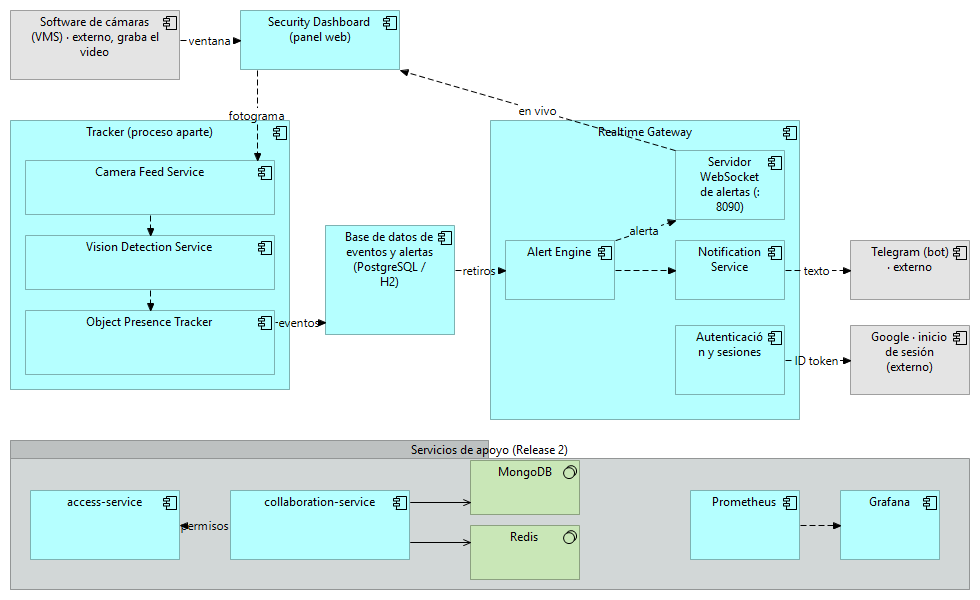
\includegraphics[width=0.82\textwidth]{../arquitectura/figuras/17-articulo.png}
\caption{Arquitectura implementada (vista ArchiMate del modelo del equipo). Gris: sistemas externos.}\label{fig:arq}
\end{figure*}

\textbf{Estilo arquitectónico y justificación.} Se combinan cuatro estilos, cada uno donde resuelve un problema concreto: \emph{tuberías y filtros}
en el procesamiento de imagen (cada etapa se prueba y se reemplaza por separado), \emph{publicación/suscripción} en las alertas (agregar un canal no toca
el motor), \emph{cliente--servidor con empuje} (el panel no consulta: recibe) y \emph{servicios pequeños con persistencia políglota} para el estado compartido,
porque tienen garantías distintas que defender. No se eligieron microservicios para todo: un equipo de tres personas y un requisito de menos de 5~s favorecen pocos
procesos; lo que escala por operadores (el gateway) se hizo sin estado para poder replicarlo, y lo que no se replica (el tracker, por cámara, junto a la pantalla)
quedó aparte.

\textbf{Decisiones técnicas relevantes.} (i) \emph{Cada motor de datos por lo que garantiza}: PostgreSQL para lo que debe ser siempre correcto (permisos,
eventos, alertas, con restricciones), MongoDB para un documento versionado y Redis solo para lo efímero; la caché \emph{muestra} pero no \emph{autoriza}
\cite{kleppmann}. (ii) \emph{Fallar cerrado}: sin base no hay sesión; sin autoridad no se guarda \cite{nygard}. (iii) \emph{Gateway sin estado}: sesiones y alertas
viven en la base, de modo que cualquier réplica atiende a cualquier operador. (iv) \emph{Configuración por variables de entorno} y valores por defecto
iguales al comportamiento anterior.

% ------------------------------------------------------------------------------------------------------------------------------------
\section{Logros técnicos del proyecto}
\subsection{Promesa de valor: tiempo real y concurrencia}
El camino de una alerta evita todo lo que suma latencia: el tracker escribe el evento, el motor lo lee cada 1~s y el WebSocket lo empuja; los avisos externos salen en
hilos aparte y la ruta crítica no depende de Redis, MongoDB ni del servicio de acceso. Medido del evento al panel: \textbf{media 0,5~s y P95 0,9~s} (meta: menos
de 5~s); confirmar un retiro toma 3 fotogramas ($\approx$2,6~s con el modelo mediano). Dos cámaras se analizan en paralelo con un seguimiento independiente por cámara.
En concurrencia, un laboratorio de consistencia mostró el defecto de partida (dos escrituras con la misma versión devolvían 200 y una se perdía) y su corrección:
con la versión en el filtro de la operación atómica de MongoDB el resultado es [200, 409]; con el permiso cacheado y la autoridad caída, la edición pasó de 200 a 503.

\subsection{Uso de IA generativa y similares}
SafeMode usa dos modelos como parte del producto: YOLOv8 local (detección y pose; visión, no generativo) y, de forma \emph{opcional}, un modelo de visión y lenguaje
de NVIDIA que redacta una descripción del dueño y de quien retira el objeto a partir de un recorte; solo se ejecuta en segundo plano, con un servidor falso en las
pruebas, y el recorte con la cara sale a un tercero, por lo que es opcional y está declarado. En el desarrollo se usó un asistente de código (Claude Code) para análisis,
código, pruebas, scripts de k6, flujos de CI, informes y documentación; el equipo revisó, ejecutó las pruebas, midió y decidió. Ningún secreto se incluyó en las
instrucciones a la IA ni en el repositorio.

\subsection{Disponibilidad y escalabilidad}
El gateway se replicó tras un balanceador con vigilancia activa (\texttt{/ready}, que comprueba la base) y pasiva. Para ello se cambió el código en tres puntos: las
alertas llegan a todas las réplicas por sondeo de la base cada 0,5~s; la creación de una alerta resiste la carrera entre réplicas (la restricción \texttt{UNIQUE} decide);
y las sesiones se guardan en la base (huella SHA-256, falla cerrada). Con dos réplicas y operadores conectados, matar una réplica (SIGKILL) produjo \textbf{0 fallos en
555 peticiones}, reconexión de los operadores en $\leq$2,1~s, ninguna alerta perdida ni duplicada y la réplica de vuelta en $\approx$5~s. Con los SLA publicados \cite{aws}, el
cálculo en serie y paralelo pasa de \textbf{99,5\,\%} (un servidor, 3,6~h de caída al mes) a \textbf{99,9375\,\%} (balanceador multi-AZ, dos gateways en dos zonas y base Multi-AZ,
27~min al mes). \emph{Límite:} el servidor público sigue siendo uno; el diseño distribuido está calculado y validado como prototipo, no desplegado.

\subsection{Rendimiento (TPS y TPM con k6)}
Se simuló un puesto real: cada operador mantiene un WebSocket y consulta sesión, cámaras y reporte, mientras un generador inserta un retiro cada 0,5~s. Se distinguen la \emph{solicitud}
(petición HTTP) y la \emph{transacción de negocio} (alerta entregada), con $\mathrm{TPS}=N_{\mathrm{trans}}/t$ y $\mathrm{TPM}=60\cdot\mathrm{TPS}$. Con 20 operadores el sistema inicial
incumplía 3 de 9 umbrales (P95 de 726~ms; \texttt{/report} de 1\,892~ms) con la CPU en 0,7 núcleos de 16: esperaba, no calculaba. La causa fue un servidor de 32 hilos con una conexión JDBC
compartida y una consulta por fila; la ley de Little \cite{little} reproduce la meseta (32 hilos / 1~s $\approx$ 32 req/s por réplica). Tras tres cambios (consultas por lotes, nombres de
cámara una vez, barrido en una consulta) se repitió la misma prueba (Tabla~\ref{tab:res} y Fig.~\ref{fig:estres}). HTTP escala hasta unos 400 operadores (678 req/s, $\approx$40\,700 TPM);
el límite pasó a la \emph{entrega de alertas}: con el umbral de 5~s el TPS sostenible es de 143 req/s y 100 alertas/s (50 operadores).

\subsection{Seguridad}
Tres escenarios, aprobados por el docente, con tácticas y validación ejecutable. \emph{ES-1} (autenticación y autorización): inicio de sesión con Google (el servidor verifica el ID
token \cite{google}), lista blanca de correos y roles en un servicio de permisos; sesión de 256 bits en cookie \texttt{HttpOnly} y \texttt{SameSite=Strict} de la que el servidor guarda solo la
huella SHA-256; 100\,\% de las rutas protegidas responden 401 sin sesión (35 pruebas). \emph{ES-2} (ataques web y ciclo de la sesión): \texttt{Origin} y \texttt{Host} exigidos a todo cambio
de estado, pool de hilos con límites de tiempo y cierre de los WebSockets al terminar la sesión. \emph{ES-3} (integridad de \texttt{/frames}): el proxy exige sesión (\texttt{forward\_auth});
12 de 12 comprobaciones reproducibles. TLS lo gestiona Caddy; las claves viven solo en variables de entorno. Brechas declaradas: cookie sin \texttt{Secure} y sin registro de auditoría.

\subsection{Mantenibilidad}
El \emph{pipeline} usa tres \emph{reusable workflows} y el despliegue depende del control de calidad. Medido con SonarQube: control de calidad en verde (cobertura del código nuevo
98,5\,\%), fiabilidad, seguridad y mantenibilidad en \textbf{A}, 0 errores y 0 vulnerabilidades, con \textbf{81,8\,\%} de cobertura de líneas en el backend (479 pruebas) y \textbf{99,3\,\%} en el
panel (144 pruebas). El análisis encontró cuatro errores reales (se corrigieron con prueba) y cuatro falsos positivos de SQL, justificados en el código; medir el panel destapó dos defectos
de interfaz. Una lección: un arreglo sin prueba hizo fallar el control (el código nuevo cuenta).

\subsection{Portabilidad}
Todo componente se ejecuta en contenedores y se configura por variables de entorno; el mismo conjunto de archivos Compose se usa en el equipo del desarrollador, en el prototipo de escalado y en
el servidor de AWS. Se evitaron servicios administrados propios de un proveedor (bases en contenedores; DNS y certificados fuera de AWS), de modo que migrar a servidores propios solo cambia
lo operativo (dominio, volumen, claves). \emph{Límite:} la migración a un servidor distinto no se ejecutó como prueba.

\subsection{Observabilidad}
El gateway y los servicios publican métricas (tráfico, latencia y errores por ruta, entrega de alertas, sockets, estado de cada dependencia); Prometheus descubre cada réplica por DNS y Grafana
muestra el tablero del equipo junto a las métricas de k6, enviadas por \emph{remote write}. Ocho reglas de alerta detectan la degradación; en las pruebas se dispararon las de \textbf{latencia} y de
\textbf{entrega}, no la de CPU: vigilar solo el recurso habría dado una falsa tranquilidad.

% ------------------------------------------------------------------------------------------------------------------------------------
\section{Resultados y validación}
\begin{table}[t]
\centering\caption{Resultados medidos antes y después de la corrección (2 réplicas).}\label{tab:res}
\footnotesize
\begin{tabular}{@{}p{3.55cm}p{1.9cm}p{1.9cm}@{}}
\toprule
\textbf{Métrica} & \textbf{Antes} & \textbf{Después} \\
\midrule
Carga: P95 HTTP (20 operadores) & 726 ms & \textbf{48 ms} \\
Carga: umbrales cumplidos & 6 de 9 & \textbf{9 de 9} \\
Carga: TPS / TPM de solicitudes & 33,3 / 2\,000 & 48,0 / 2\,882 \\
Pico (20$\rightarrow$300): req/s de promedio & 25 & \textbf{217} \\
Pico: P95 HTTP & 10,3 s & \textbf{0,6 s} \\
Estrés: meseta HTTP (req/s) & 34--48 & \textbf{570--678} \\
Estrés: alertas entregadas & 5\,967 & \textbf{185\,756} \\
Estrés: P95 de toda la prueba & 15,7 s & 2,2 s \\
\bottomrule
\end{tabular}
\end{table}

\begin{table*}[t]
\centering\caption{Atributos de calidad: escenario, medida y resultado.}\label{tab:atributos}
\footnotesize
\begin{tabular}{@{}p{2.3cm}p{5.3cm}p{4.6cm}p{4.6cm}@{}}
\toprule
\textbf{Atributo} & \textbf{Escenario (estímulo $\rightarrow$ respuesta)} & \textbf{Medida comprometida} & \textbf{Resultado medido} \\
\midrule
Tiempo real & Un objeto se retira $\rightarrow$ el panel muestra la alerta & Menos de 5 s extremo a extremo & Evento$\rightarrow$panel: media 0,5 s, P95 0,9 s \\
Rendimiento & 20 operadores; estrés hasta 600; pico 20$\rightarrow$300 & P95 $<$ 500 ms; errores $<$ 1\,\%; TPS $\geq$ 40 & P95 48 ms; 0\,\%; 48 req/s; meseta 570--678 req/s \\
Disponibilidad y escalabilidad & Una réplica del gateway cae de golpe con tráfico & 0 peticiones fallidas; reconexión $\leq$ 2,1 s & 0 de 555 fallidas; 2,07 s; vuelve en 5 s; 99,5 $\rightarrow$ 99,9375\,\% (calculado) \\
Seguridad & Sin cuenta o cuenta ajena; ataque web; frames falsos & 401/403 en toda ruta protegida; 0 frames no autenticados & 35 pruebas (ES-1); pruebas ES-2; 12 de 12 (ES-3) \\
Mantenibilidad & Un \texttt{push} al repositorio & Cobertura $\geq$ 80\,\%; calificación A; control verde & 81,8\,\% y 99,3\,\%; A, A, A; verde (código nuevo 98,5\,\%) \\
Portabilidad & Mover el sistema de AWS a servidores propios & 0 líneas de código cambiadas; todo en contenedores & Mismo Compose en tres entornos (límite: sin migración ejecutada) \\
Observabilidad & Una dependencia cae o la latencia sube & Detección en $\leq$ 1 min; cada dependencia publica su estado & 8 reglas; se dispararon latencia y entrega \\
Concurrencia & Dos escrituras con la misma versión; permiso revocado & Una gana (200), otra 409; sin permiso verificable, 503 & Antes [200, 200]; después [200, 409] y 503 \\
\bottomrule
\end{tabular}
\end{table*}

\begin{figure}[t]
\centering
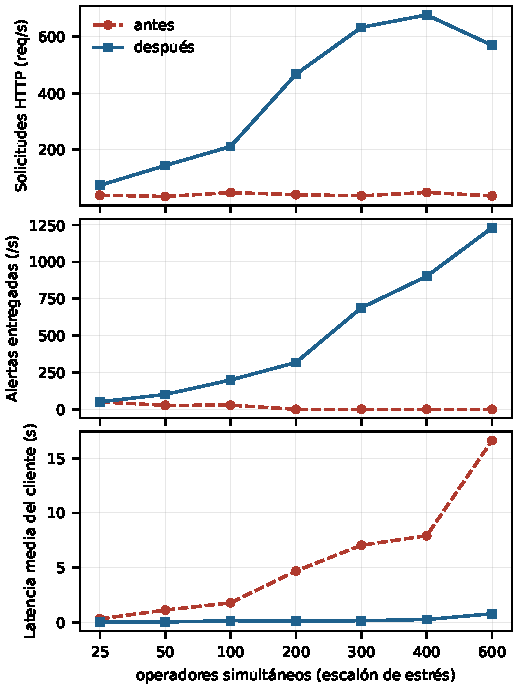
\includegraphics[width=\columnwidth]{figuras/estres-comparacion.pdf}
\caption{Estrés con 2 réplicas por escalón de operadores, antes y después de la corrección.}\label{fig:estres}
\end{figure}

Las gráficas del cliente se calculan por ventana a partir de los contadores de k6 (que exporta percentiles acumulados) y se verificaron contra el resumen de k6: la misma media, las mismas solicitudes, las
mismas alertas y los mismos errores en las seis corridas. \textbf{Amenazas a la validez.} Todo corrió en un solo equipo con el generador incluido (cifras relativas, no la capacidad de la instancia de
AWS); el generador es de ciclo cerrado; la base no se vació entre corridas (cada una empezó con más alertas pendientes que la anterior, lo que hace \emph{conservadora} la mejora), y el estrés
posterior empezó con 2\,446 alertas pendientes frente a 1\,028 del anterior; el P95 de entrega de toda la prueba no es comparable entre corridas con muy distinta cantidad de alertas entregadas.
El código, los scripts y los resultados de k6 y de las demás pruebas están versionados y son reproducibles (commit \texttt{\versionrepo}).

% ------------------------------------------------------------------------------------------------------------------------------------
\section{Conclusiones}
\textbf{Lo aprendido.} Medir antes de suponer: la CPU no era el límite, lo era una conexión compartida con consultas repetidas, y la medición lo mostró. Cada motor de datos por lo que
garantiza, y una caché que muestra pero no autoriza, evitaron las fallas de consistencia que el laboratorio reprodujo. Declarar los límites aumenta la credibilidad.

\textbf{Impacto arquitectónico.} Tres decisiones explican la mayoría de los resultados: el gateway sin estado (replicable sin tocar su lógica), la persistencia políglota con fallo
cerrado, y las interfaces en los puntos de variación (fuente de fotogramas, sesión, verificación del token, canal de avisos).

\textbf{Limitaciones.} Despliegue público de un solo servidor; la entrega de alertas pasa de 5~s con 100 operadores o más; el tracker es un punto único de detección; pendientes el aviso por correo,
la prueba con dos cámaras físicas y la corrida en SonarCloud; resultados de rendimiento de un solo equipo.

\textbf{Trabajo futuro.} Pool de conexiones y \emph{snapshot} acotado para la entrega de alertas; desplegar el diseño distribuido y repetir las pruebas con el generador en otra máquina; cerrar las
brechas de seguridad (cookie \texttt{Secure}, auditoría); y completar los pendientes del producto.

% ------------------------------------------------------------------------------------------------------------------------------------
\begin{thebibliography}{99}
\bibitem{bass} L. Bass, P. Clements y R. Kazman, \emph{Software Architecture in Practice}, 4.\textsuperscript{a} ed. Boston, MA, EE.\,UU.: Addison-Wesley, 2021.
\bibitem{archimate} The Open Group, \emph{ArchiMate 3.2 Specification}, 2022.
\bibitem{scrum} K. Schwaber y J. Sutherland, \emph{The Scrum Guide}, 2020. [En línea]. Disponible: \url{https://scrumguides.org}
\bibitem{adr} M. Nygard, ``Documenting architecture decisions,'' 2011. [En línea]. Disponible: \url{https://cognitect.com/blog/2011/11/15/documenting-architecture-decisions}
\bibitem{docker} Docker Inc., ``Compose file reference.'' [En línea]. Disponible: \url{https://docs.docker.com/compose/}
\bibitem{sonar} SonarSource, ``SonarQube documentation: quality gates.'' [En línea]. Disponible: \url{https://docs.sonarsource.com/sonarqube/}
\bibitem{k6} Grafana Labs, ``k6 documentation.'' [En línea]. Disponible: \url{https://grafana.com/docs/k6/latest/}
\bibitem{prom} Prometheus Authors, ``Prometheus documentation.'' [En línea]. Disponible: \url{https://prometheus.io/docs/}
\bibitem{yolo} G. Jocher, A. Chaurasia y J. Qiu, ``Ultralytics YOLOv8,'' 2023. [En línea]. Disponible: \url{https://github.com/ultralytics/ultralytics}
\bibitem{little} J. D. C. Little, ``A proof for the queuing formula: $L=\lambda W$,'' \emph{Operations Research}, vol. 9, n.\textsuperscript{o} 3, pp. 383--387, 1961.
\bibitem{kleppmann} M. Kleppmann, \emph{Designing Data-Intensive Applications}. Sebastopol, CA, EE.\,UU.: O'Reilly, 2017.
\bibitem{nygard} M. T. Nygard, \emph{Release It!}, 2.\textsuperscript{a} ed. Raleigh, NC, EE.\,UU.: Pragmatic Bookshelf, 2018.
\bibitem{google} Google, ``Verify the Google ID token on your server side.'' [En línea]. Disponible: \url{https://developers.google.com/identity/gsi/web/guides/verify-google-id-token}
\bibitem{aws} Amazon Web Services, ``Service Level Agreements'' de Amazon EC2, Elastic Load Balancing y Amazon RDS, consultados el 19 de noviembre de 2026. [En línea]. Disponible: \url{https://aws.amazon.com/legal/service-level-agreements/}
\end{thebibliography}

\end{document}
